\section{Volumenkontrol}

\begin{frame}{Volumenkontrol}
\scriptsize{
\begin{table}[h]
\centering
\begin{tabular}{l|r}
\hline\hline
Område & Krav \\
\hline\hline
Frekvensgang & < 0,375 dB ved 20 Hz - 20 kHz, ref. 1 kHz \\
& < 0,75 dB fra 20 Hz til 63 Hz \\
& < 0,75 dB fra 12,5 kHz til 20 kHz \\[4pt]
Dæmpningsområde i & 0 - 50 dB ved 1 kHz \\
volumenkontrol & \\[4pt]
Styring af volumen- & Digital \\
kontrol & \\[4pt]
Antal niveauer i & 51 \\
volumenkontrollen & \\[4pt]
Dæmpning per & 1 dB \\
niveau & \\[4pt]
Input fra brugeren & To trykknapper \\[4pt]
Output til brugeren & To 7-segmenter \\
\hline\hline
\end{tabular}
%\caption{Krav til volumenkontrollen}
%\label{tab:krav_volumenkontrol}
\end{table}}
\end{frame}

\begin{frame}{Volumenkontrol}
\begin{figure}[h]
\centering
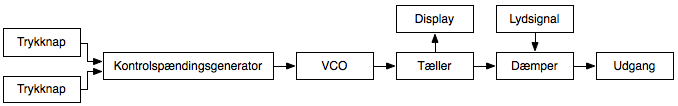
\includegraphics[scale=0.4]{images/blokdiagram-volumenkontrol.png}
%\caption{Overordnet blokdiagram over volumenkontrollen}
%\label{fig:blokdiagram_volumenkontrol}
\end{figure}
%\end{frame}

%\begin{frame}{Volumenkontrol}
\begin{itemize}
\item<2-> Kontrolspændingsgenerator
\item<3-> VCO
\item<4-> Tæller
\item<5-> Display
\item<6-> Dæmper
\end{itemize}
\end{frame}